% Hasse diagram of the 2 x 2 factorial design with repeated measures used by
% the ISA round-trip fixture (examples/isa-roundtrip/). Supplementary figure
% for issue #35; not \input by main.tex. Compile standalone:
%   pdflatex hasse-2x2-design.tex
%
% Each node is a factor of the design, with its number of levels. An edge goes
% from a coarser factor to a finer one that it contains. Day enters the fitted
% model (STATO linear mixed model) as a linear term, with a random intercept per
% animal: activity_count ~ treatment * enrichment + day; random intercept: animal.
\documentclass[border=6pt]{standalone}
\usepackage{tikz}
\usetikzlibrary{positioning,arrows.meta}
\begin{document}
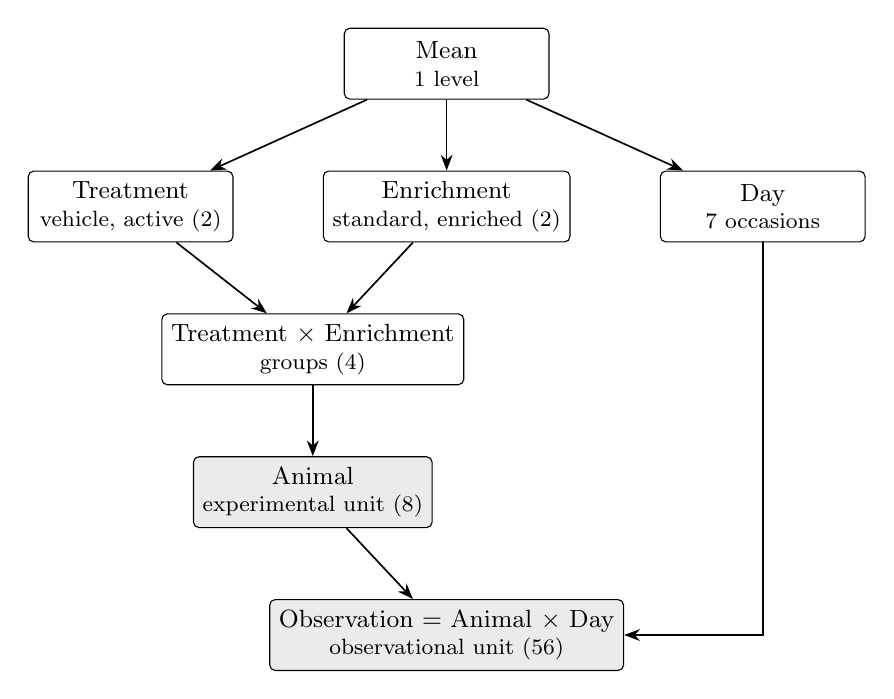
\begin{tikzpicture}[
    every node/.style={draw, rounded corners=2pt, align=center, font=\small,
                       minimum width=26mm, minimum height=9mm},
    unit/.style={fill=black!8},
    edge/.style={-{Stealth[length=2mm]}, semithick},
    node distance=9mm and 6mm]
  \node (mean) {Mean\\[-1pt]\footnotesize 1 level};

  \node (trt) [below left=of mean, xshift=-8mm] {Treatment\\[-1pt]\footnotesize vehicle, active (2)};
  \node (enr) [below=of mean] {Enrichment\\[-1pt]\footnotesize standard, enriched (2)};
  \node (day) [below right=of mean, xshift=8mm] {Day\\[-1pt]\footnotesize 7 occasions};

  \node (te) [below=of enr, xshift=-17mm] {Treatment $\times$ Enrichment\\[-1pt]\footnotesize groups (4)};
  \node (animal) [unit, below=of te] {Animal\\[-1pt]\footnotesize experimental unit (8)};
  \node (obs) [unit, below=of animal, xshift=17mm] {Observation = Animal $\times$ Day\\[-1pt]\footnotesize observational unit (56)};

  \draw[edge] (mean) -- (trt);
  \draw[edge] (mean) -- (enr);
  \draw[edge] (mean) -- (day);
  \draw[edge] (trt) -- (te);
  \draw[edge] (enr) -- (te);
  \draw[edge] (te) -- (animal);
  \draw[edge] (animal) -- (obs);
  \draw[edge] (day) |- (obs);
\end{tikzpicture}
\end{document}
